\begin{exercise}
(Ramificaciones)

\begin{itemize}
    \item Describa (de manera similar a lo hecho en clase) las superficies de Riemann asociadas a las siguientes funciones. Esto es, haga un listado de los puntos de ramificación, el índice u orden de la ramificación y los cortes y pegados requeridos para construir la superficie de Riemann.
    $$z^{2/3}, \qquad \sqrt {(z^2 -1) (z^2 - 4)}, \qquad \sqrt[3] {z^3 - z}, \qquad \sqrt {z^3 - 3z},$$
    $$\log(z), \qquad \log(z^2 + i), \qquad z^{5/7} (z-3)^{2/7}$$
    
    \item (Dessin d'enfant versión Coquito: \url{https://mathoverflow.net/questions/1909/})
    
    Un \textit{dessin d'enfant} es una representación esquemática de un cubrimiento ramificado $\pi : X \to \widehat \C$ que tiene a lo más tres puntos de ramificación. Mediante una transformación de Möbius de $\widehat \C$, podemos suponer que los puntos de ramificación son $0, 1, \infty$.
    
    El dessin d'enfant de $\pi$ es un grafo en el cual
    \begin{itemize}
        \item Los puntos de $\pi^{-1}(0)$ se representan como vértices blancos.
        \item Los puntos de $\pi^{-1}(1)$ se representan como vértices negros.
        \item Las componentes conexas de $\pi^{-1}((0, 1))$ se representan como aristas rojas que unen un vértice blanco con un vértice negro.
        \item El encaje del grafo en $X$ es parte íntegra de la estructura.
    \end{itemize}
    
    Para toda superficie de Riemann $X$, las siguientes proposiciones son equivalentes:
    \begin{itemize}
        \item $X$ es la complejificación de una curva algebraica proyectiva no singular sobre $\bar \Q$.
        \item $X$ es el espacio base de un cubrimiento ramificado $\pi : X \to \widehat \C$ que tiene a lo más tres puntos de ramificación.
    \end{itemize}
    
    Este resultado demostrado por Belyi explica la importancia \textit{aritmética} de los dessins d'enfant, pues estos últimos nos dan una herramienta \textit{geométrica} para investigar la estructura del grupo de Galois absoluto $\Gal(\Q)$, un objeto muy importante, pero poco comprendido hasta el momento.
    
    Bajo estas consideraciones, se le pide que
    \begin{itemize}
        \item Construya un dessin d'enfant para las funciones $f_n : \C \to \C$ definidas por $f_n(z) = z^n$.
        \item Construya un dessin d'enfant para las funciones $g_1, g_2 : \C \to \C$ definidas por
        $$g_1(z) = \frac {27} 4 z^2 (1-z), \qquad \qquad g_2(z) = 16 z^2 (1 - z)^2$$
        
        \item Halle una función holomorfa $h(z)$ cuyo dessin d'enfant sea
        \begin{figure}[h]
            \centering
            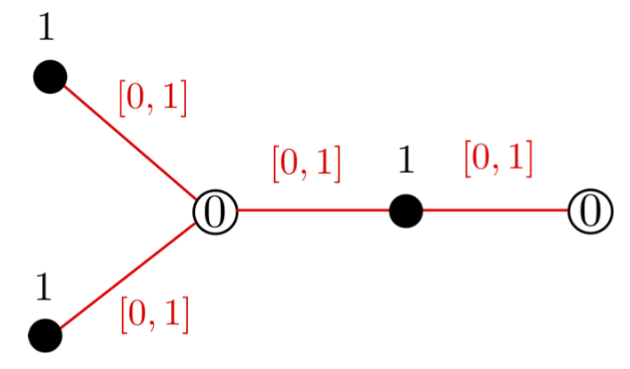
\includegraphics[scale=0.25]{dessins/example.png}
            \caption{Esquema de $h(z)$.}
        \end{figure}
        
        \item Construya un dessin d'enfant para $T_n^2(z)$, donde $T_n(z)$ es el $n$-ésimo polinomio de Chebyshev y está definido por $T_n(\cos \theta) = \cos(n\theta)$.
    \end{itemize}
\end{itemize}
\end{exercise}

\begin{solution}
\leavevmode
\begin{itemize}
    \item En todos los casos, la superficie de Riemann en cuestión está definida por una ecuación de la forma $f(z) = g(w) = u$, donde $g$ tiene un único punto de ramificación en el origen. Entonces,
    \begin{itemize}
        \item Los puntos de la superficie de Riemann están determinados por sus coordenadas $z, w$. Por ende, la superficie buscada es el pullback que cierra universalmente el diagrama conmutativo
        $$
        \begin{tikzcd}[row sep=large, column sep=large]
            X \arrow[r, dashed] \arrow[d, dashed] & \C_z \arrow[d, "f"] \\
            \C_w \arrow[r, "g"] & \C_u
        \end{tikzcd}
        $$
        donde $\C_z, \C_w, \C_u$ son los planos con coordenadas $z, w, u$, respectivamente.
        
        \item Puesto que el único punto de ramificación de $g^{-1}$ es el origen de $\C_u$, podemos tomar una curva que pasa por el origen de $\C_u$ para definir las ramas. Hemos escogido el eje real $\Im(u) = 0$, que divide el plano $\C_u$ en dos regiones que colorearemos rosa y celeste.
        \begin{figure}[h]
            \centering
            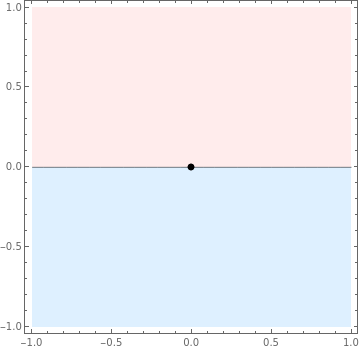
\includegraphics[scale=0.4]{ramification/0-u.png}
            \caption{El plano $\C_u$ con el único punto de ramificación de $g^{-1}$.}
        \end{figure}
        
        \item En ningún caso se puede graficar directamente la superficie de Riemann buscada. Para superar este impasse, graficaremos las proyecciones de la superficie sobre $\C_z, \C_w$. Las preimágenes de la recta $\Im(u) = 0$ dividen a estos planos en regiones que serán pintadas con el mismo color que su imagen en $\C_u$.
        
        \item El método más simple posible para construir cada superficie de Riemann es 
        \begin{itemize}
            \item Tomar tantas copias de $\C_z$ como haya ramas de $g^{-1}$ y ordenarlas cíclicamente.
            \item Cortar todas las copias a lo largo de la curva $\Im(f(z)) = 0$.
            \item Considerar los tramos en la curva $\Im(f(z)) = 0$ cuyos extremos son puntos de ramificación y/o críticos de $w(z)$. Determinar en qué dirección se debe cruzar el tramo para avanzar a la siguiente rama.
            \item Dado un lazo $\gamma$ que cruza la curva $\Im(f(z)) = 0$ sin pasar por ningún punto de ramificación, definir la cantidad auxiliar
            
            
            $$n(\gamma) = \sum_{z \in R_f} W(\gamma, z)$$
            donde $R_f \subset \C_z$ es el conjunto de puntos de ramificación de $f$ y $W(\gamma, z)$ es la cantidad de vueltas (\textit{winding number}) que $\gamma$ da alrededor de $z \in R$.
            \item El levantamiento de $\gamma$ a la superficie es un camino que avanza $n(\gamma)$ ramas de $w(z)$.
        \end{itemize}
        
        Este método hace muchos más cortes que los estrictamente necesarios, pero tiene la ventaja de que siempre funciona y no hay que pensar demasiado para aplicarlo.
    \end{itemize}
    
    Sin más preámbulo...
    
    \begin{enumerate}[label=\alph*)]
        \item El único punto de ramificación de $w(z) = z^{2/3}$ es el origen $z = 0$, con índice de ramificación $3$.
        \begin{figure}[h]
            \centering
            \begin{subfigure}{.4\textwidth}
                \centering
                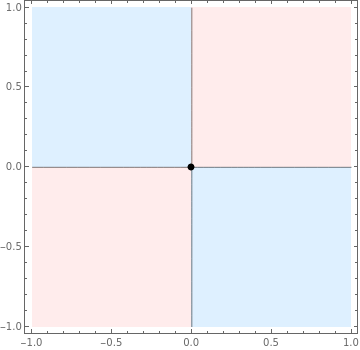
\includegraphics[scale=0.35]{ramification/1-z.png}
            \end{subfigure}
            \begin{subfigure}{.4\textwidth}
                \centering
                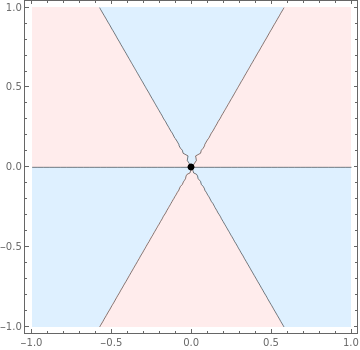
\includegraphics[scale=0.35]{ramification/1-w.png}
            \end{subfigure}
            \caption{Los planos $\C_z, \C_w$, donde $w^3 = z^2$.}
        \end{figure}
        
        Para construir la superficie de Riemann buscada:
        \begin{itemize}
            \item Tomemos tres copias de $\C_z$, ordenadas cíclicamente y cortadas el eje real negativo.
            \item Peguemos el lado superior del eje real negativo en cada copia con el lado inferior del mismo eje real negativo en la siguiente copia.
        \end{itemize}
        
        Observemos que el espacio construido tiene una singularidad en el origen. Siendo estrictos, una superficie de Riemann es, primero y ante todo, una variedad diferenciable. Entonces, para tener una superficie de Riemann propiamente dicha, debemos eliminar el origen. Otra posibilidad es resolver la singularidad mediante una explosión (\textit{blowup}).
        
        \item Los puntos de ramificación de $w(z) = \sqrt {(z^2 - 1) (z^2 - 4)}$ son los ceros del radicando, colocados en  los puntos $z = \pm 1$, $z = \pm 2$. En todos los casos, el índice de ramificación es $2$.
        \begin{figure}[h]
            \centering
            \begin{subfigure}{.4\textwidth}
                \centering
                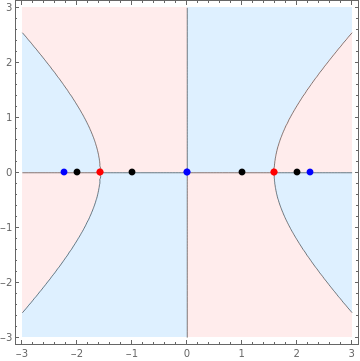
\includegraphics[scale=0.4]{ramification/2-z.png}
            \end{subfigure}
            \begin{subfigure}{.4\textwidth}
                \centering
                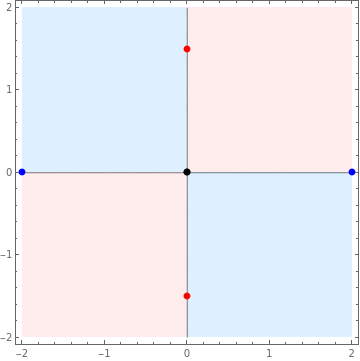
\includegraphics[scale=0.4]{ramification/2-w.png}
            \end{subfigure}
            \caption{Los planos $\C_z, \C_w$, donde $w^2 = (z^2 - 1) (z^2 - 4)$.}
        \end{figure}
        
        Observemos que
        \begin{itemize}
            \item Cruzar el segmento $A = [1, 2]$ o su espejo $B = [-2, -1]$ en $\C_z$ equivale a girar alrededor del origen en el plano $\C_w$, dentro del rombo con vértices en $z = \pm 2$, $z = \pm 3i/2$.
            
            \item Para $z \gg 0$, tenemos $w^2 \approx z^4$. Puesto que $2$ divide a $4$, no hay ramificación en el infinito. Entonces, los cortes se pueden hacer a lo largo de segmentos compactos.
        \end{itemize}
        
        Para construir la superficie de Riemann buscada,
        \begin{itemize}
            \item Tomemos dos copias de $\C_z$, cortadas en los segmentos $A, B$.
            \item Peguemos el lado superior de cada segmento cortado ($A, B$) con el lado inferior del mismo segmento en la otra copia de $\C_z$.
        \end{itemize}
        
        \item Los puntos de ramificación de $w(z) = \sqrt [3] {z^3 - z}$ son los ceros del radicando, que están colocados en los puntos $z = 0$, $z \pm 1$. En todos los casos, el índice de ramificación es $3$.
        \begin{figure}[h]
            \centering
            \begin{subfigure}{.4\textwidth}
                \centering
                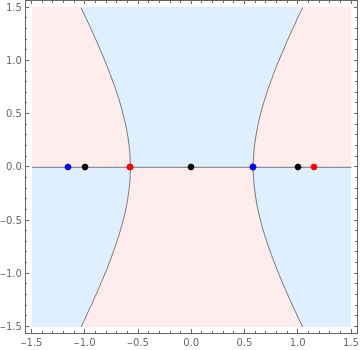
\includegraphics[scale=0.4]{ramification/3-z.png}
            \end{subfigure}
            \begin{subfigure}{.4\textwidth}
                \centering
                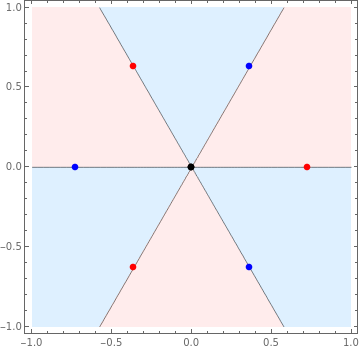
\includegraphics[scale=0.4]{ramification/3-w.png}
            \end{subfigure}
            \caption{Los planos $\C_z, \C_w$, donde $w^3 = z^3 - z$.}
        \end{figure}
        
        Observemos que
        \begin{itemize}
            \item Cruzar el segmento $A = [-1, 1]$ en el plano $\C_z$ equivale a girar alrededor del origen en $\C_w$, dentro del hexágono con vértices en las raíces sextas de la unidad.
            
            \item Para $z \gg 0$, tenemos $w^3 \approx z^3$. Puesto que $3$ divide a $3$, no hay ramificación en el infinito. Entonces los cortes se pueden hacer a lo largo de segmentos compactos.
        \end{itemize}
        
        Para construir la superficie de Riemann buscada,
        \begin{itemize}
            \item Tomemos tres copias de $\C_z$, llamadas $\C_1, \C_2, \C_3$.
            \item Cortemos cada plano $\C_k$ en los segmentos $A_{1k} = [-1, 0]$ y $A_{2k} = [0, 1]$.
            \item Peguemos el lado superior de $A_{jk}$ con el lado inferior de $A_{jl}$, donde $l = j + k \pmod 3$.
        \end{itemize}
        
        \item Los puntos de ramificación de $w(z) = \sqrt {z^3 - 3z}$ son los ceros del radicando, que están colocados en los puntos $z = 0$, $z = \pm \sqrt 3$. En todos los casos, el índice de ramificación es $2$.
        \begin{figure}[h]
            \centering
            \begin{subfigure}{.4\textwidth}
                \centering
                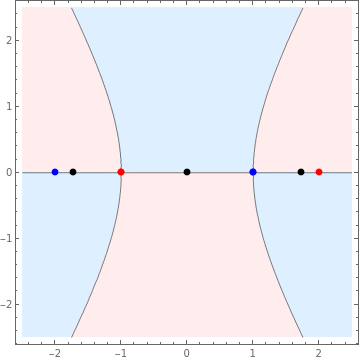
\includegraphics[scale=0.4]{ramification/4-z.png}
            \end{subfigure}
            \begin{subfigure}{.4\textwidth}
                \centering
                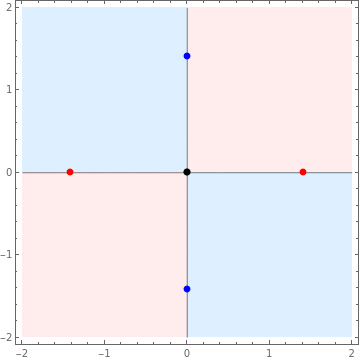
\includegraphics[scale=0.4]{ramification/4-w.png}
            \end{subfigure}
            \caption{Los planos $\C_z, \C_w$, donde $w^2 = z^3 - 3z$.}
        \end{figure}
        
        Observemos que
        \begin{itemize}
            \item Para $z \gg 0$, tenemos $w^2 \approx z^3$. Puesto que $2$ no divide a $3$, hay ramificación en el infinito. Entonces debemos hacer algún corte no acotado.
        \end{itemize}
        
        Para construir la superficie de Riemann buscada:
        \begin{itemize}
            \item Tomemos dos copias de $\C_z$, cortadas en los segmentos $A = [-1, 0]$ y $B = [1, \infty)$.
            \item Peguemos el lado superior de cada segmento cortado ($A, B$) con el lado inferior del mismo segmento en la otra copia de $\C_z$.
        \end{itemize}
        
        \item El único punto de ramificación de $\log(z)$ es el origen $z = 0$, con índice de ramificación $\infty$. Esta vez ocurren dos cosas que no veíamos en las curvas algebraicas:
        \begin{itemize}
            \item La función no tiene puntos críticos.
            \item El punto de ramificación no está en el dominio de la función.
        \end{itemize}
        
        Por ende, no tenemos suficientes puntos de referencia como en los ítems anteriores. Para mitigar este inconveniente, hemos graficado explícitamente los cortes en los planos $\C_z, \C_w$.
        \begin{figure}[h]
            \centering
            \begin{subfigure}{.4\textwidth}
                \centering
                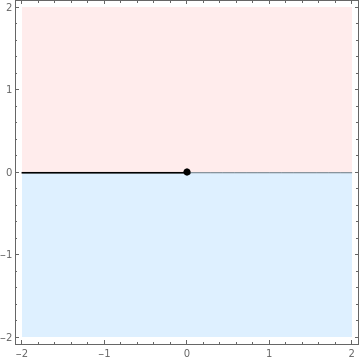
\includegraphics[scale=0.4]{ramification/5-z.png}
            \end{subfigure}
            \begin{subfigure}{.4\textwidth}
                \centering
                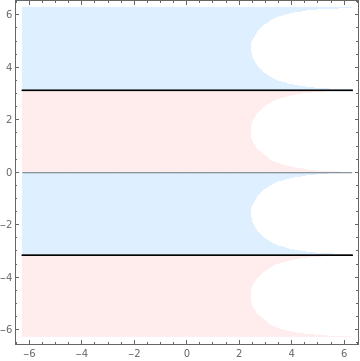
\includegraphics[scale=0.4]{ramification/5-w.png}
            \end{subfigure}
            \caption{Los planos $\C_z, \C_w$, donde $e^w = z$.}
        \end{figure}
        
        Debemos pensar que la imagen de $z = 0$ es un punto extra $w = -\infty$ situado muy a la izquierda del plano $\C_w$. Para construir la superficie de Riemann buscada:
        \begin{itemize}
            \item Tomemos infinitas copias de $\C_z^\star$, indizadas por los enteros $\Z$.
            \item Cortemos cada copia de $\C_z^\star$ en el eje real negativo.
            \item Peguemos el lado superior del eje real negativo en cada copia con el lado inferior del mismo eje real negativo en la siguiente copia.
        \end{itemize}
        
        El resultado de este proceso es el recubrimiento universal del plano agujereado $\pi : X \to \C_z^\star$, que es biholomorfo al plano complejo usual $\C_w$. Podemos pensar en $X$ como una hélice infinita que proyecta sombra sobre el plano agujereado.
        \begin{figure}[h]
            \centering
            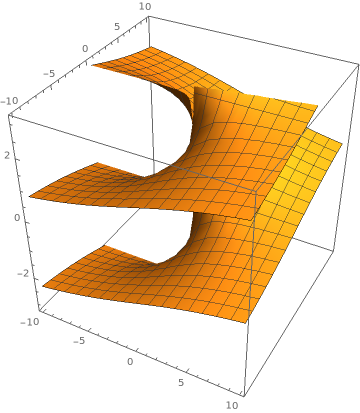
\includegraphics[scale=0.5]{ramification/5-helix.png}
            \caption{El recubrimiento universal $\pi : X \to \C_z^\star$.}
        \end{figure}
        
        \item En este ítem, no cortaremos el plano $\C_u$ a lo largo del eje real $\Im(u) = 0$, sino a lo largo del eje imaginario $\Re(u) = 0$. La razón detrás de esta elección será clara más adelante. El eje $\Re(u) = 0$ también divide a $\C_u$ en dos regiones que colorearemos rosa y celeste.
        \begin{figure}[h]
            \centering
            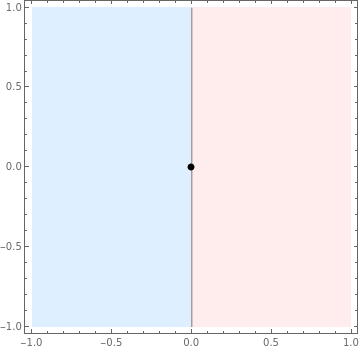
\includegraphics[scale=0.4]{ramification/6-u.png}
            \caption{El plano $\C_u$ cortado a lo largo de un eje diferente.}
        \end{figure}
        
        Los puntos de ramificación de $w(z) = \log(z^2 + i)$ son los ceros de la expresión suministrada a la función logaritmo, i.e., $z = \pm \sqrt {-i}$. En ambos casos, el índice de ramificación es $\infty$.
        \begin{figure}[h]
            \centering
            \begin{subfigure}{.4\textwidth}
                \centering
                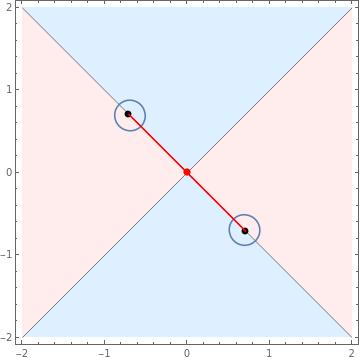
\includegraphics[scale=0.4]{ramification/6-z.png}
            \end{subfigure}
            \begin{subfigure}{.4\textwidth}
                \centering
                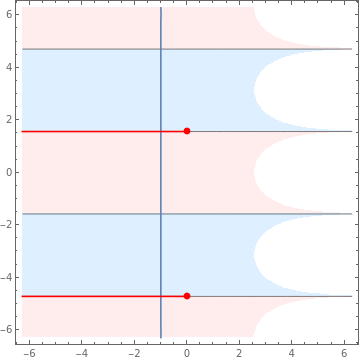
\includegraphics[scale=0.4]{ramification/6-w.png}
            \end{subfigure}
            \caption{Los planos $\C_z, \C_w$, donde $e^w = z^2 + i$.}
        \end{figure}
        
        La ventaja del corte en $\C_u$ a lo largo de $\Re(u) = 0$ es que el corte $\Re(z^2 + i) = 0$ inducido en $\C_z$ pasa por los puntos de ramificación de $w(z)$. Entonces podemos usar este corte para realizar la transición de una rama del logaritmo a la siguiente.
        
        (De hecho, la única razón por la cual utilizamos el corte $\Im(u) = 0$ en los ítems anteriores es que en dichos casos $f(z)$ era un polinomio con raíces reales.)
        
        Para construir la superficie de Riemann buscada:
        \begin{itemize}
            \item Tomemos infinitas copias de $\C_z$, indizadas por los enteros $\Z$.
            
            \item Cortemos cada copia de $\C_z$ a lo largo del segmento que conecta a las raíces de $z^2 + i$. Esto equivale a cortar $\C_w$ a lo largo de los rayos que parten de $2\pi in$ y se extienden de manera horizontal en el semiplano izquierdo.
            
            \item Peguemos el lado superior del segmento cortado en una copia de $\C_z$ con el lado inferior del segmento cortado en la siguiente copia de $\C_z$. Esto equivale a pegar las ramas de la función logaritmo de la manera usual.
        \end{itemize}
        
        El resultado de este proceso es una superficie de Riemann suave, sin puntos singulares. Esto se debe a que $g$ no tiene puntos críticos. Por ende, al menos de manera local, $w$ se puede expresar como una función holomorfa de $z$.
        
        \item Los puntos de ramificación de $w(z) = \sqrt [7] {z^5 (z-3)^2}$ son los ceros del radicando, colocados en los puntos $z = 0$ y $z = 3$. En ambos casos, el índice de ramificación es $7$.
        \begin{figure}[h]
            \centering
            \begin{subfigure}{.4\textwidth}
                \centering
                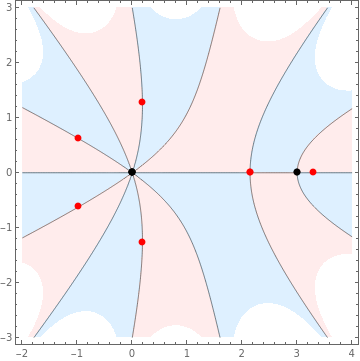
\includegraphics[scale=0.4]{ramification/7-z.png}
            \end{subfigure}
            \begin{subfigure}{.4\textwidth}
                \centering
                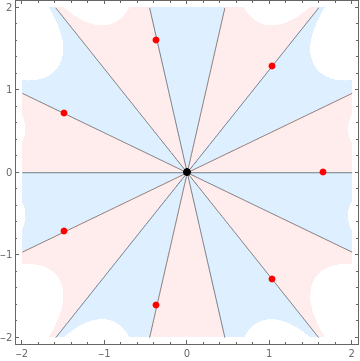
\includegraphics[scale=0.4]{ramification/7-w.png}
            \end{subfigure}
            \caption{Los planos $\C_z, \C_w$, donde $w^7 = z^5 (z-3)^2$.}
        \end{figure}
        
        Observemos que
        \begin{itemize}
            \item Cruzar el segmento $A = [0, 3]$ equivale a girar alrededor del origen en el plano $\C_w$, dentro del heptágono con vértices en las raíces séptimas de la unidad.
            
            \item Para $z \gg 0$, tenemos $w^7 \approx z^7$. Puesto que $7$ divide a $7$, no hay ramificación en el infinito. Entonces los cortes se pueden hacer a lo largo de segmentos compactos.
        \end{itemize}
        
        Para construir la superficie de Riemann buscada:
        \begin{itemize}
            \item Tomemos siete copias de $\C_z$, ordenadas cíclicamente.
            \item Cortemos cada copia de $\C_z$ a lo largo del segmento $[0, 3]$.
            \item Peguemos el lado superior del segmento cortado en una copia de $\C_z$ con el lado inferior del segmento cortado en la siguiente copia de $\C_z$.
        \end{itemize}
        
        Puede parecer sorprendente que no hayamos tenido cuidado de pasar a la quinta o a la segunda copia más adelante en el orden cíclico. Sin embargo, esto no es problema, pues tanto $5$ como $2$ son relativamente primos a $7$ y, por ende, generan el grupo cíclico $\Z / 7\Z$ que indiza las copias.
    \end{enumerate}
    
    \item Para generar los dessins d'enfant, utilicé la siguiente rutina en Mathematica:
    \begin{lstlisting}[language=Mathematica]
    diag = 1 + I;
    size = PointSize[0.02];
    proc[f_, a_, b_] := Module[{p0, p1, p2, p3, p4, sol},
        sol[t_] := z /. Solve[f == t];
        p0 = ComplexContourPlot[Im[f], {z, a - b*diag, a + b*diag},
            Contours -> {0}, ContourStyle -> Red, ContourShading -> False];
        p1 = ComplexListPlot[sol[-1], PlotStyle -> {Red, size}];
        p2 = ComplexListPlot[sol[0], PlotStyle -> {Blue, size}];
        p3 = ComplexListPlot[sol[1], PlotStyle -> {Black, size}];
        p4 = ComplexListPlot[sol[2], PlotStyle -> {Red, size}];
        Show[p0, p1, p4, p2, p3]
    ];
    \end{lstlisting}
    
    El parámetro principal de esta rutina es una función holomorfa $f : \C \to \C$. La rutina grafica
    \begin{itemize}
        \item La preimagen del eje real como una curva roja.
        \item La preimagen de $-1$ como una colección de puntos rojos.
        \item La preimagen de $0$ como una colección de puntos azules. (Blancos, en el enunciado.)
        \item La preimagen de $1$ como una colección de puntos negros.
        \item La preimagen de $2$ como una colección de puntos rojos.
    \end{itemize}
    
    El propósito de marcar los puntos rojos es simplemente indicar qué partes de la curva roja deben ser ignoradas. Los segmentos que nos interesan unen a puntos azules con puntos negros. Finalmente, los parámetros auxiliares $a, b$ controlan el posicionamiento de la gráfica de una manera más conveniente que la utilizada por Mathematica por defecto.
    
    Sin más preámbulo...
    
    \begin{itemize}
        \item El dessin d'enfant de la función $z^n$ es una estrella con un único punto blanco (el origen) unido por segmentos rojos a $n$ puntos negros (las $n$ raíces de la unidad).
        
        \item El dessin d'enfant de $g_1$ se construye con el comando
        \begin{lstlisting}[language=Mathematica]
        g1 = 27/4*z^2*(1 - z);
        proc[g1, 1/3, 1 + I]
        \end{lstlisting}
        
        Obtenemos el siguiente resultado:
        \begin{figure}[h]
            \centering
            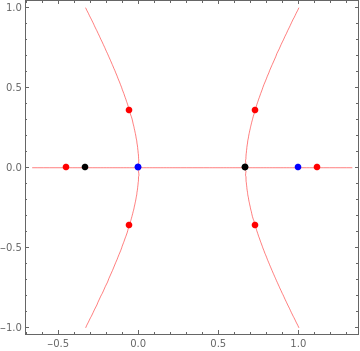
\includegraphics[scale=0.4]{dessins/g1.png}
            \caption{Esquema de $g_1(z)$.}
        \end{figure}
        
        Ignorando los tramos que pasan por los puntos rojos, el dessin d'enfant de $g_1$ es un camino que pasa por puntos negro blanco, negro, blanco, en sucesión.
        
        \item El dessin d'enfant de $g_2$ se construye con el comando
        \begin{lstlisting}[language=Mathematica]
        g2 = 16*z^2*(1 - z)^2;
        proc[g2, 1/2, 1 + I]
        \end{lstlisting}
        
        Obtenemos el siguiente resultado:
        \begin{figure}[h]
            \centering
            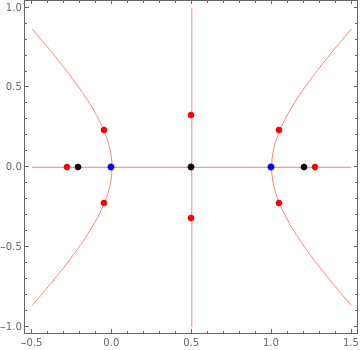
\includegraphics[scale=0.4]{dessins/g2.png}
            \caption{Esquema de $g_2(z)$.}
        \end{figure}
        
        Ignorando los tramos que pasan por los puntos rojos, el dessin d'enfant de $g_2$ es un camino que pasa por puntos negro, blanco, negro, blanco, negro, en sucesión.
        
        \item Puesto que el dessin d'enfant dado es un árbol (no tiene ciclos), podemos asumir que $h(z)$ es un polinomio. Como los puntos $t \in (0, 1)$ no son de ramificación, ellos ilustran el comportamiento genérico de la ecuación $h(z) = t$. Entonces,
        \begin{itemize}
            \item $h(z)$ es un polinomio de grado $4$.
            \item $h(z)$ tiene una raíz triple.
            \item $1 - h(z)$ tiene una raíz doble.
        \end{itemize}
        
        Parece razonable hacer los siguientes supuestos adicionales:
        \begin{itemize}
            \item Las raíces de $h(z)$ son reales.
            \item Las raíces simples de $1 - h(z)$ son complejos conjugados.
        \end{itemize}
        
        Jugando con Mathematica, encontré la función $h(z) = 16 z^3 (2 - 3z)$. Posteriormente me dijeron en \url{https://math.stackexchange.com/q/3668144/4675} que $h(z)$ es un reescalamiento de un polinomio de Shabat. Podemos ver que
        $$1 - h(z) = (1 - 2z)^2 (1 + 4z + 12z^2)$$
        tiene una raíz real doble y dos raíces complejas conjugadas, como predijimos inicialmente. Para construir el dessin d'enfant de $h(z)$, utilizamos el siguiente comando:
        \begin{lstlisting}[language=Mathematica]
        h = 16*z^3 (2 - 3 z);
        proc[h, 1/4, 1 + I]
        \end{lstlisting}
        
        Obtenemos el siguiente resultado:
        \begin{figure}[h]
            \centering
            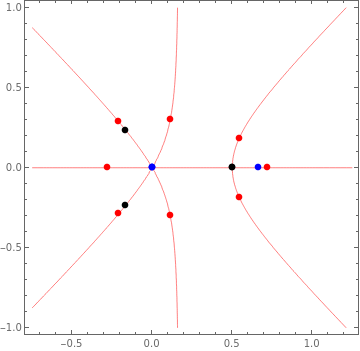
\includegraphics[scale=0.4]{dessins/h.png}
            \caption{Esquema de $h(z)$.}
        \end{figure}
        
        Ignorando los tramos que pasan por los puntos rojos, el dessin d'enfant de $h$ tiene la forma de árbol que se indica en el enunciado.
        
        \item Las siguientes afirmaciones se demuestran de manera tediosa pero fácil por inducción:
        \begin{itemize}
            \item $\cos(n \theta)$, $\sin(n \theta)$ son polinomios homogéneos de grado $n$ en $\cos \theta$, $\sin \theta$.
            \item $\sin \theta$ aparece con exponente par en todos los términos de $\cos(n \theta)$.
            \item $\sin \theta$ aparece con exponente impar en todos los términos de $\sin(n \theta)$.
        \end{itemize}
        
        Sustituyendo $\sin^2(z) = 1 - \cos^2(z)$ en la expansión de $\cos(nz)$, demostramos que $\cos(nz)$ es un polinomio de grado $n$ en $\cos(z)$. Este polinomio es $T_n(z)$. Además,
        \begin{itemize}
            \item Las soluciones de $\cos^2(n \theta) = 0$ son los ángulos $\theta \in S^1$ tales que $e^{in\theta} = \pm i$. Estas soluciones vienen en pares complejos conjugados. Por ende, $T^2(z)$ tiene $n$ raíces distintas, cada una de multiplicidad $2$.
            
            \item Las soluciones de $\sin^2(n \theta) = 0$ son los ángulos $\theta \in S^1$ tales que $e^{in\theta} = \pm 1$. Estas soluciones vienen en pares complejos conjugados, a excepción de $\pm 1$. Por ende, $1 - T^2(z)$ tiene $n+1$ raíces disitntas: $z = \pm 1$, ambas de multiplicidad $1$, y todas las demás de multiplicidad $2$.
        \end{itemize}
        
        Por ende, el dessin d'enfant de $T_n^2(z)$ es un único segmento en el que aparecen $2n+1$ nodos de colores alternados, empezando y terminando con un nodo negro.
        
        Para confirmar este hallazgo, graficamos los dessins d'enfant de $T_n^2(z)$ para $n = 2,3,4,5$:
        \begin{lstlisting}
        cheb[n_] := ChebyshevT[n, z]^2;
        proc[cheb[2], 0, 1]
        proc[cheb[3], 0, 1]
        proc[cheb[4], 0, 1]
        proc[cheb[5], 0, 1]
        \end{lstlisting}
        
        Obtenemos el siguiente resultado:
        \begin{figure}[h]
            \centering
            \begin{subfigure}{.4\textwidth}
                \centering
                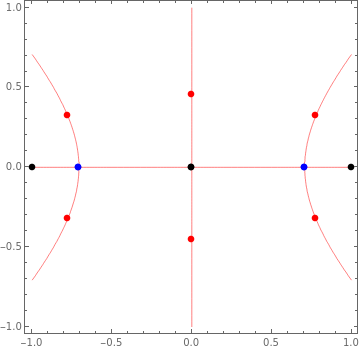
\includegraphics[scale=0.4]{dessins/t2.png}
            \end{subfigure}
            \begin{subfigure}{.4\textwidth}
                \centering
                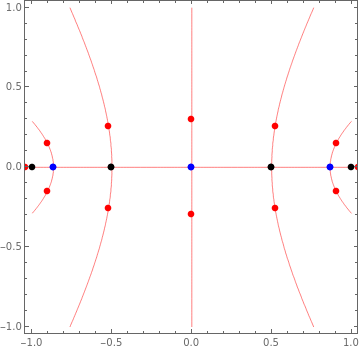
\includegraphics[scale=0.4]{dessins/t3.png}
            \end{subfigure}
            \begin{subfigure}{.4\textwidth}
                \centering
                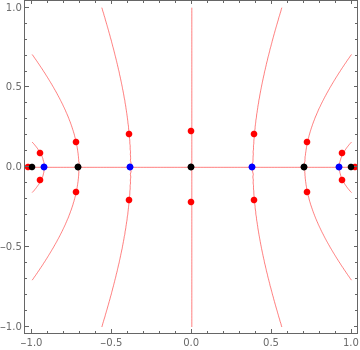
\includegraphics[scale=0.4]{dessins/t4.png}
            \end{subfigure}
            \begin{subfigure}{.4\textwidth}
                \centering
                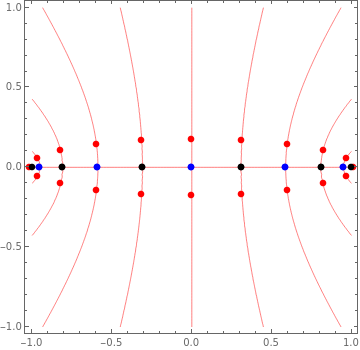
\includegraphics[scale=0.4]{dessins/t5.png}
            \end{subfigure}
            \caption{Esquema de $T_n^2(z)$ para $n = 2,3,4,5$.}
        \end{figure}
    \end{itemize}
\end{itemize}
\end{solution}
